\documentclass{beamer}

\makeatletter
\def\input@path{%
    {../components/}%
}%
\makeatother

\definecolor{crtBlack}{rgb}{.1,.07,.06}
\definecolor{crtWhite}{rgb}{.87,.87,.98}
\definecolor{crtGreen}{rgb}{.22,.93,.05}
\setbeamercolor{normal text}{fg=crtWhite,bg=crtBlack}
\setbeamercolor{structure}{fg=crtGreen}
\setbeamerfont{structure}{family=\ttfamily}
% \setbeamerfont{title}{size=\Large}


\usepackage{cmll}
\usepackage{multirow}
\usepackage{booktabs}

\usepackage[style=authoryear]{biblatex}
\addbibresource{../text-based-worlds.bib}
\setbeamertemplate{bibliography item}{\insertbiblabel}

\AtEveryBibitem{
    \clearlist{language}
    \clearfield{month}
    \clearfield{series}
    \clearfield{venue}
    \clearname{editor}
    \clearlist{publisher}
    \clearlist{location} % alias to field 'address'
    \clearfield{doi}
    \clearfield{url}
    \clearfield{venue}
    \clearfield{issn}
    \clearfield{isbn}
    \clearfield{urldate}
    \clearfield{urlyear}
    \clearfield{urlmonth}
    \clearfield{urlday}
    \clearfield{eventdate}
    \clearfield{pages}
    %\clearfield{booktitle}
    %\clearfield{journaltitle}
    %\clearfield{number}
    %\clearfield{volume}
}

\usepackage{caption}

\usepackage{hyperref}
\hypersetup{
    pdfpagemode=FullScreen,
}

\title{Knowledge-based Solutions to Text-based Worlds}
\subtitle{Final Presentation}
\author{Morgan Wajda-Levie}
\date{May 18, 2022}

\newcommand{\game}[1]{\emph{#1}}

\begin{document}

\begin{frame}
    \titlepage
\end{frame}


% Problem description and goals
\section{Problem Description and Goals}

\begin{frame}
    \frametitle{Abstract}
    Text-based games, also called text adventures or interactive
    fiction, are a form of parser-driven text-based worlds where players
    control a Player Character in an immersive environment. Players
    interact with the environment by issuing text commands such as, ``go
    west'' or ``unlock the door with the bronze key'' and the game gives
    feedback in the form of natural language scene descriptions, e.g.
    ``You are standing in an open field west of a white house, with a
    boarded front door'' (Zork, Infocom, 1981). I would like to use
    pre-trained GloVe word embeddings to aid in parsing scene
    descriptions and action exploration, and, which in turn will be used
    to train a knowledge base that will be used for goal completion,
    with the hope that this will allow for effective knowledge transfer
    between a wide array of text adventure games.
\end{frame}

\begin{frame}[b]
    \begin{figure}
        \centering
        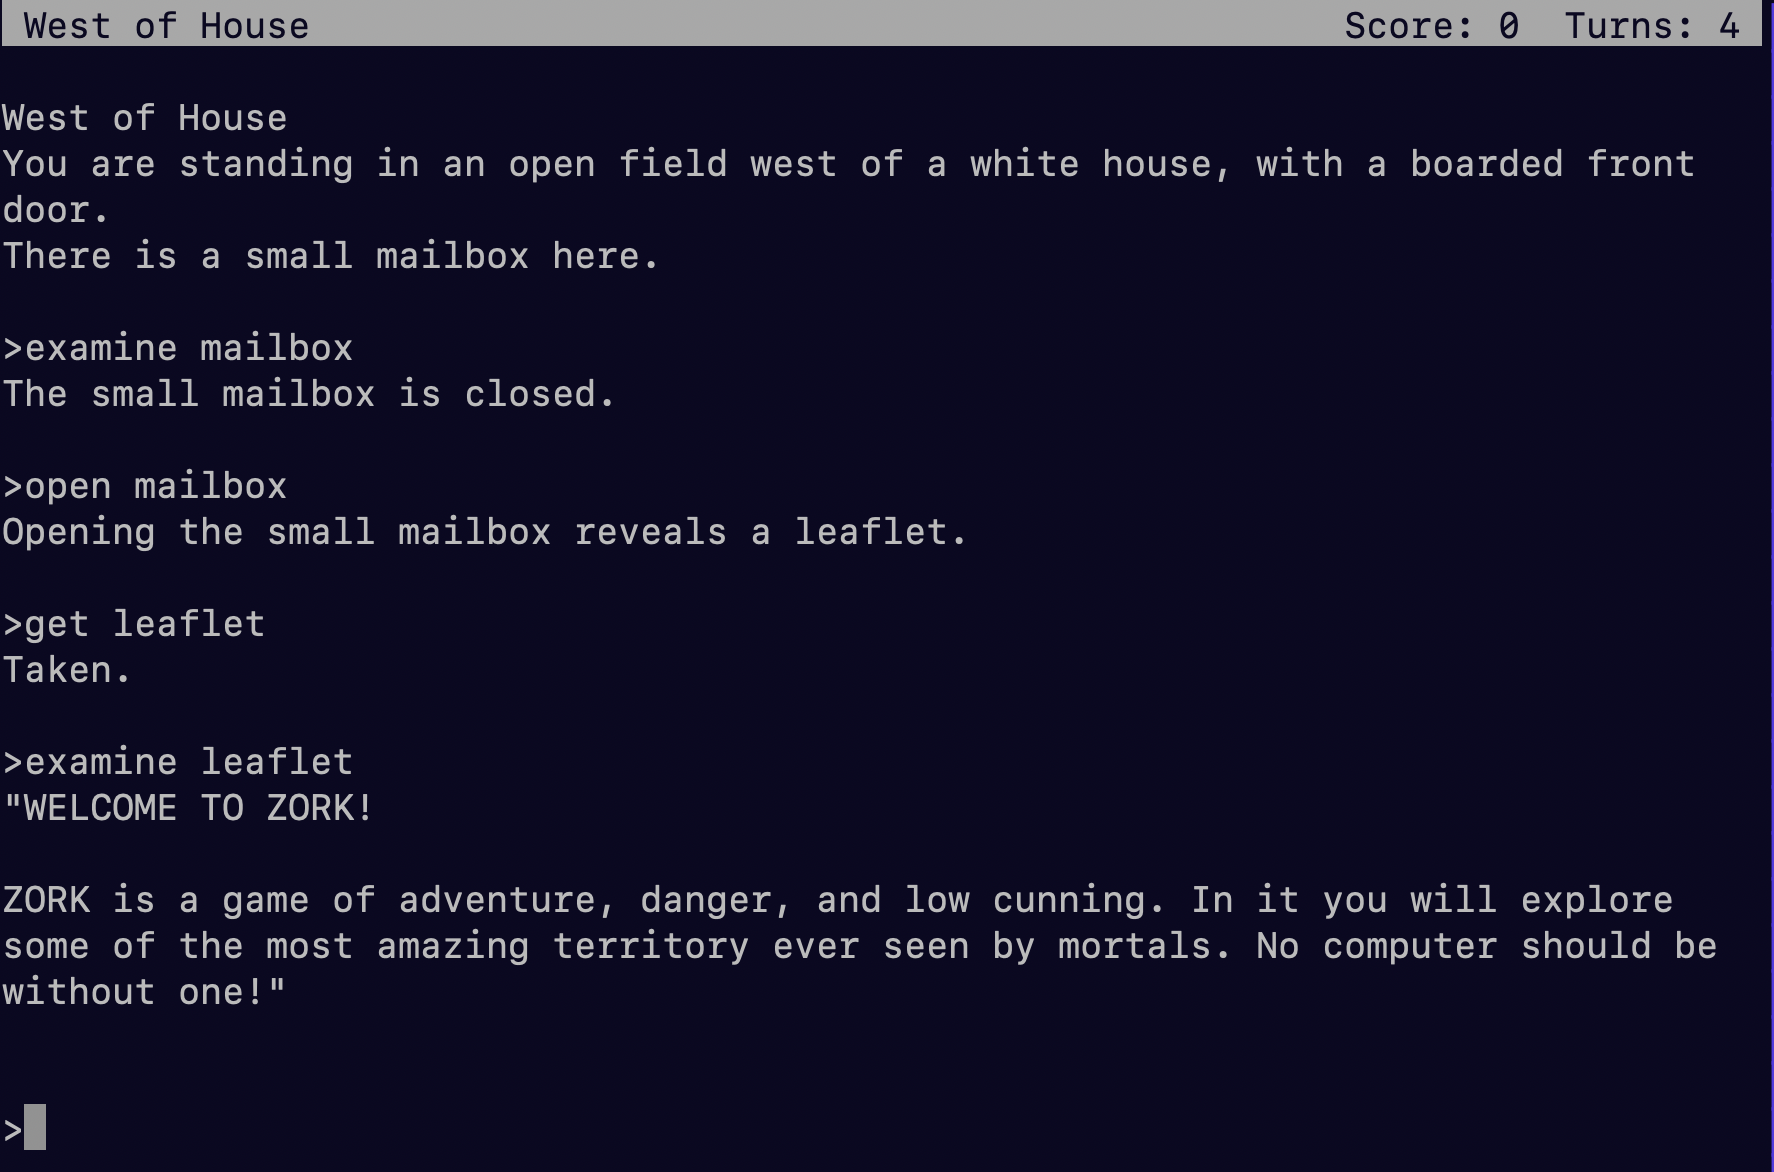
\includegraphics[width=\textwidth,keepaspectratio]{../images/zork1.png}
        \caption*{Zork I, Marc Blank and Dave Lebling, 1980}
    \end{figure}
\end{frame}

\begin{frame}[b]
    \begin{figure}
        \centering
        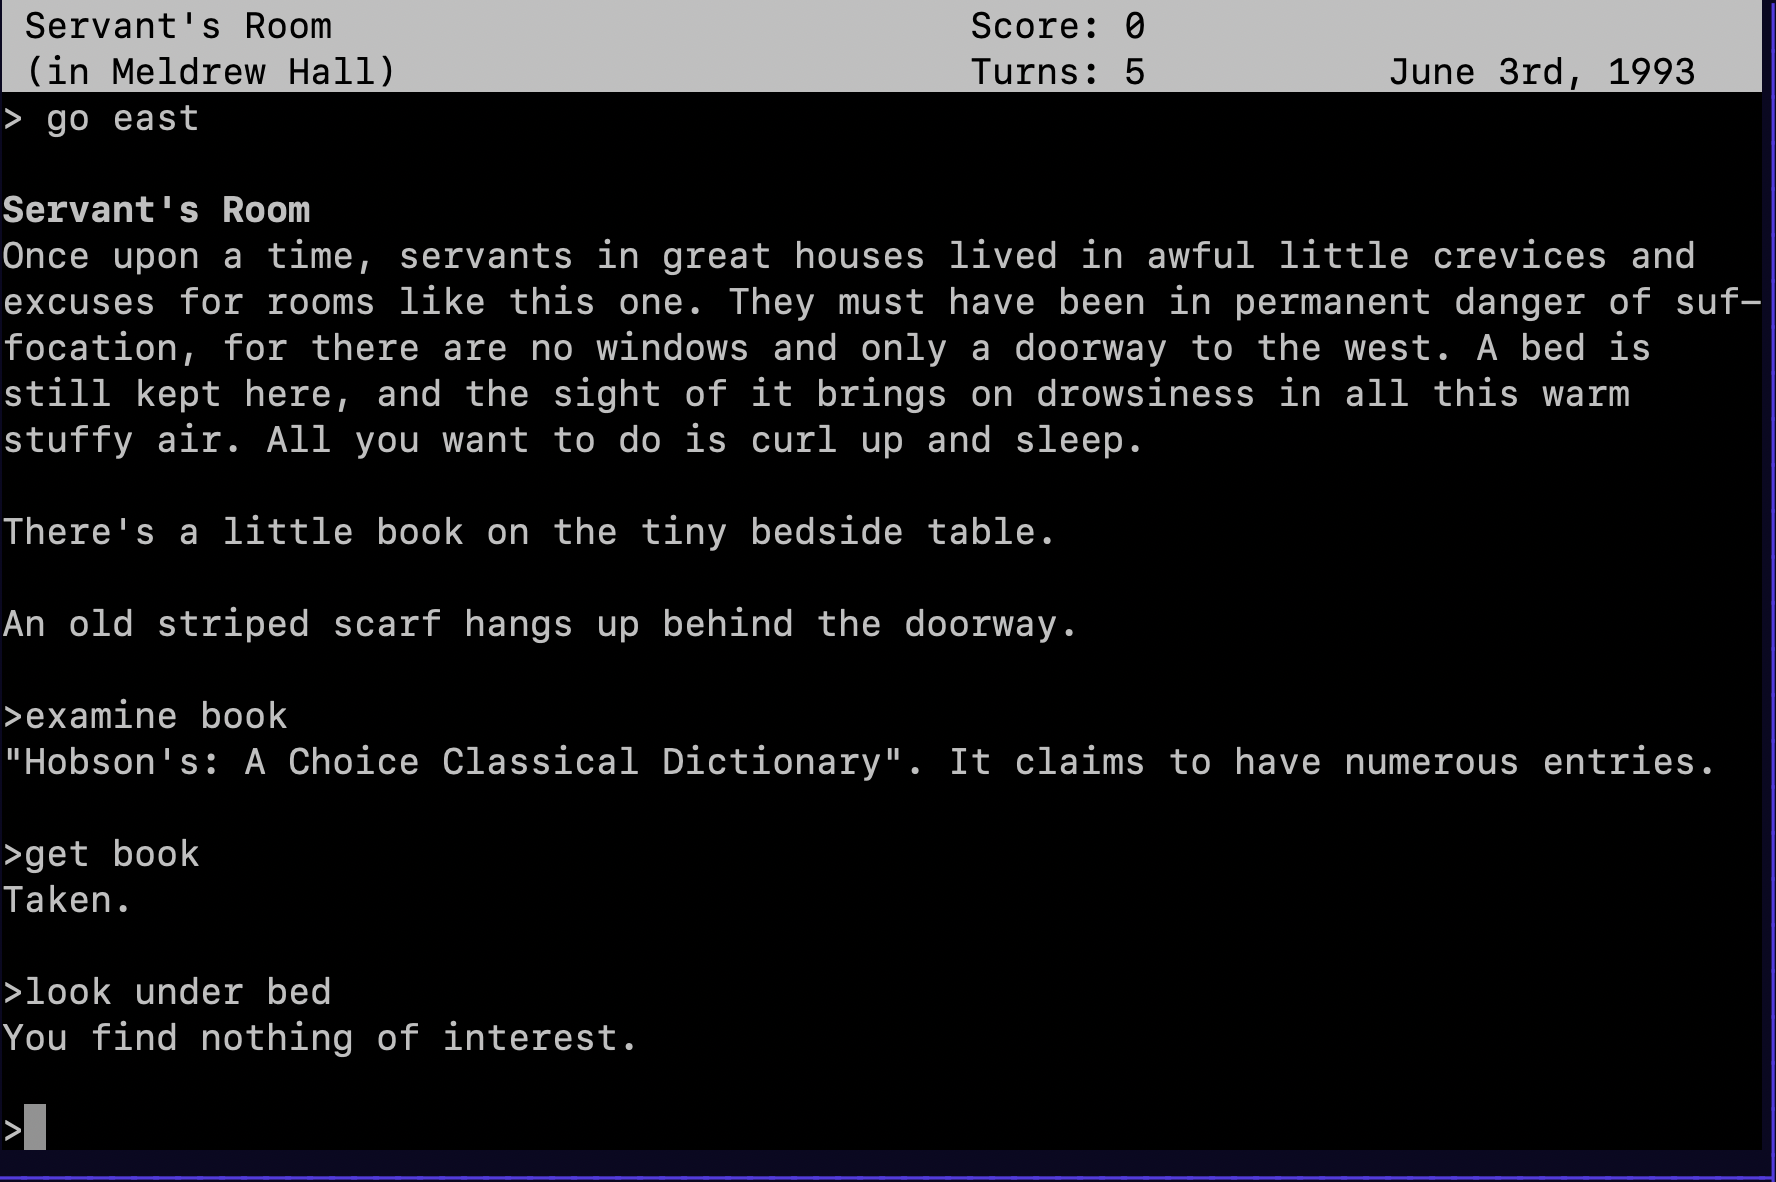
\includegraphics[width=\textwidth,keepaspectratio]{../images/curses.png}
        \caption*{Curses, Graham Nelson, 1993}
    \end{figure}
\end{frame}

\begin{frame}[b]
    \begin{figure}
        \centering
        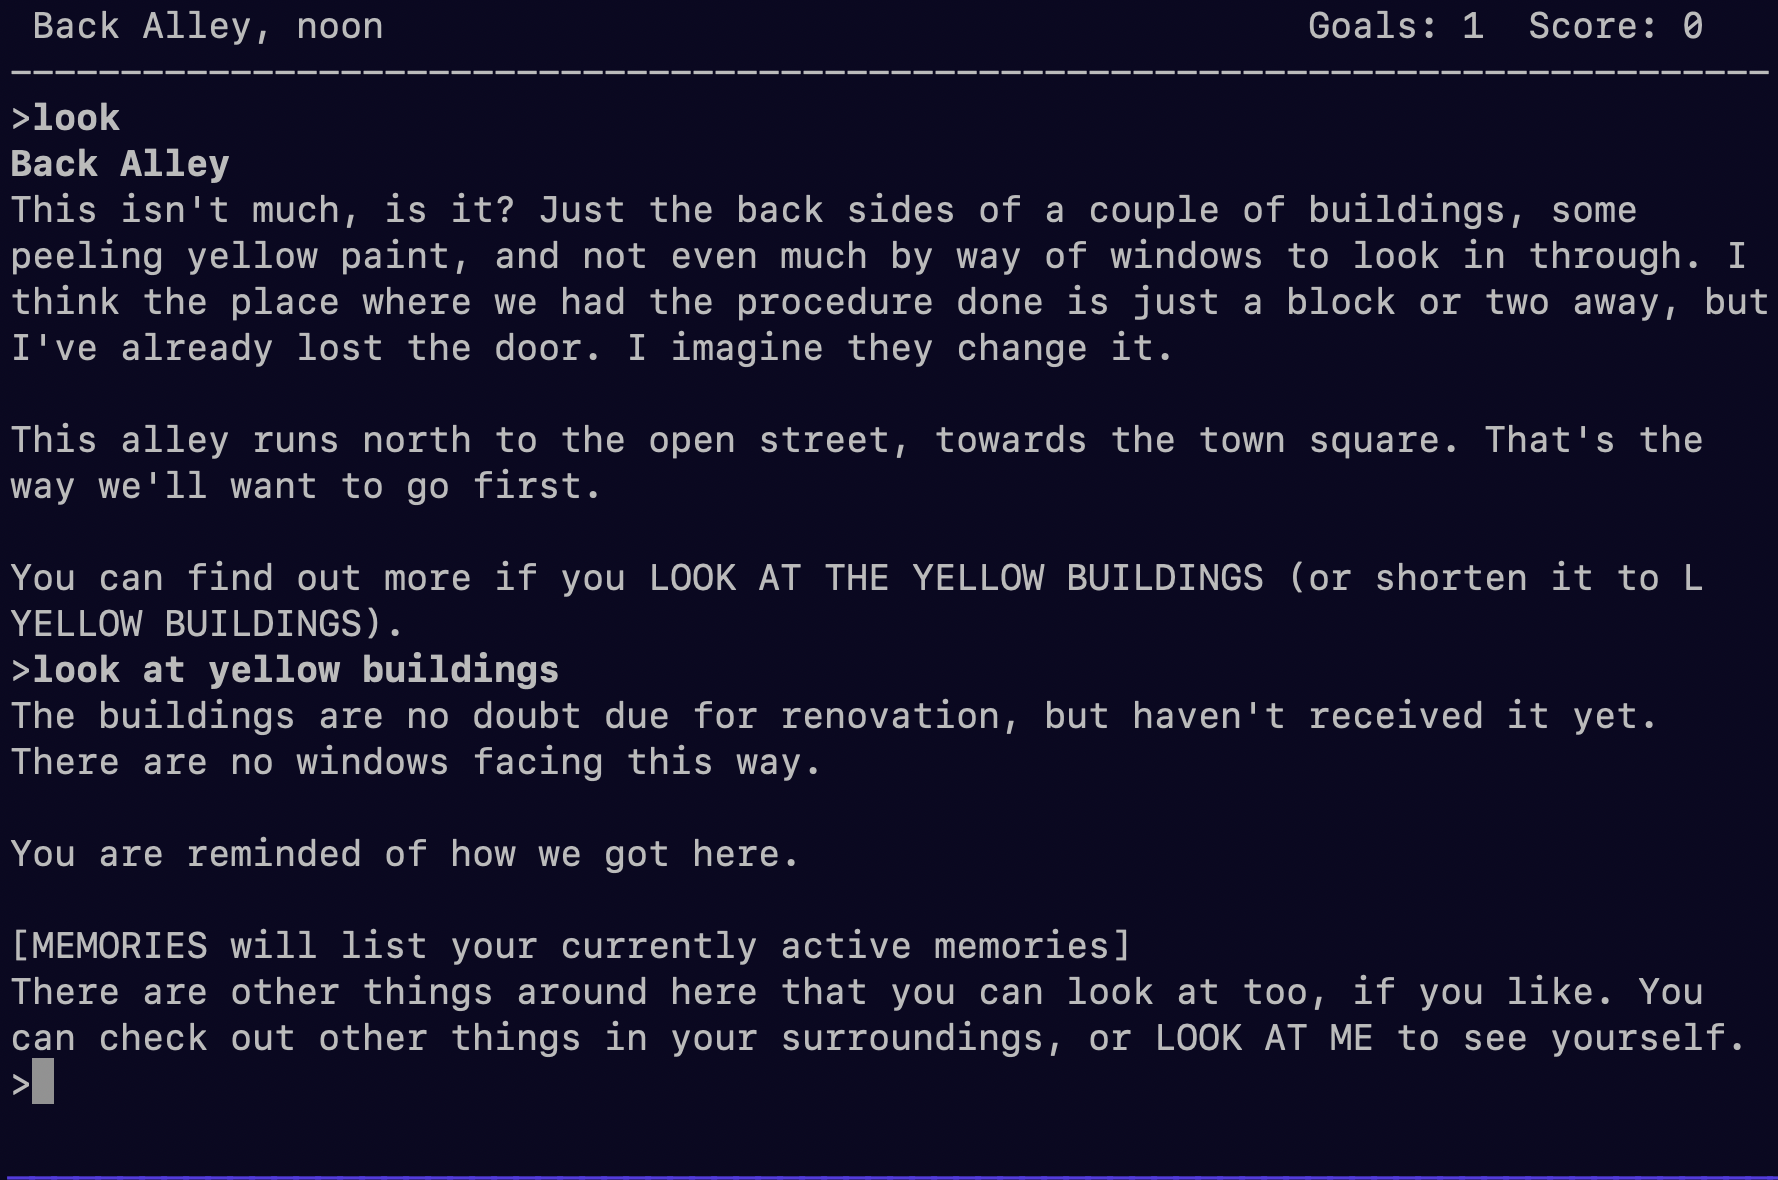
\includegraphics[width=\textwidth,keepaspectratio]{../images/counterfeit_monkey.png}
        \caption*{Counterfeit Monkey, Emily Short, 2012}
    \end{figure}
\end{frame}

\begin{frame}

    \frametitle{Text adventure games}
    \begin{columns}
    % timeline of popular games
        \column{.5\textwidth}
        \begin{block}{Popular games}
            {\footnotesize
            \begin{itemize}
                \item \game{Adventure}, William Crowther and Donald
                    Woods, 1976.
                \item \game{Zork I}, Mark Blank and Dave Lebling, 1980.
                \item \game{Enchanted}, Mark Blank and Dave Lebling,
                    1983.
                \item \game{The Hitchiker's Guide to the Galaxy},
                    Douglas Adams and Steve Meretsky, 1984.
                \item \game{Curses}, Graham Nelson, 1993.
                \item \game{Spider and Web}, Andrew Plotkin, 1998.
                \item \game{Counterfeit Monkey}, Emily Short, 2012.
            \end{itemize}
            \parencite{interactive_fiction_technology_foundation_interactive_nodate}
        }
        \end{block}

        % characteristics of games
        \column{.5\textwidth}
        \begin{block}{Common characteristics}
            \begin{itemize}
                \item Players take on the role of a character in an
                    immersive world
                \item A goal, or \emph{quest} is usually given at the
                    start of the game
                \item Players interact with the world by issuing natural
                    language commands
                \item Information about the world is conveyed to the
                    player through prose descriptions
            \end{itemize}
        \end{block}
    \end{columns}

\end{frame}

\begin{frame}

    \frametitle{An AI agent to solve mazes in text-based worlds}

    Traditional text adventures remain largely unsolvable by AI agents,
    but constrained benchmark games can be created that allow agents to
    focus on specific skills.

    \begin{block}{Goal: Design an agent to solve increasingly
        complex mazes}
        \begin{enumerate}
            \item Trivial mazes (interconnected areas without obstacles) 
            \item Simple obstacles such as doors
            \item Composite obstacles such as locked doors
            \item Stretch goal: complex, novel obstacles
        \end{enumerate}

        Wherever possible, pursue an approach that favors generalization
        and interpretability.

    \end{block}

\end{frame}

% State of the art / related work
\section{State-of-the-art and related work}

\begin{frame}

    \frametitle{Existing text-based game agents}
    \begin{description}
        \item[BYUAgent]

            Extracts nouns from game text and combines them with
            pre-generated verb list, with the help of word embeddings.
            Stores verb/noun combinations that produce a result. Winner
            of IEEE CIG 2016 Text-based adventure AI competition.
        \item[Golovin]

            Operates in one of 5 command generator modes, based on
            current game environment. Uses word embeddings trained
            on text-based game walkthroughs, tutorials and narrative
            fiction.
        \item[NAIL]

            Independent modules compete for control of the agent based
            on \emph{eagerness}. Uses a knowledge graph to track world
            state. Relies on heavily tuned command sets common to
            text-based games. Winner of IEEE CIG 2018 Text-based AI
            competition.
    \end{description}
    (\cite{atkinson_text-based_2019}, \cite{ricks_byu-agent-2016_2019},
    \cite{hausknecht_nail_2019})

\end{frame}

\begin{frame}
    \frametitle{AI frameworks for text-based games}
    \begin{description}
        \item[Jericho]

            A python-based library for using learning agents with
            text-based games.
            \parencite{hausknecht_interactive_2020}
        \item[TextWorld]
            
            A python-based library for procedurally generating
            text-based games.
            \parencite{cote_textworld_2019}
    \end{description}
\end{frame}

% Approach
\section{Approach}

\begin{frame}
    \frametitle{Approach}

    \begin{block}{Priorities: Generalizable and interpretable}
        \begin{itemize}
            \item Favor generalizable knowledge (e.g. keys unlock doors)
                over genre-tuned heuristics
            \item Favor interpretable algorithms over deep neural
                networks
        \end{itemize}
    \end{block}

    \begin{block}{NLP-assisted groupings in hierarchical knowledge
        base}
        \begin{itemize}
            \item Crude parsing of scene descriptions using word
                embeddings
            \item Use knowledge base to encode observations of objects
                in rooms
            \item Using word embeddings, navigate a hierarchical
                knowledge base tying observations of verbs applied to
                objects to look for matches
            \item Exploit strong matches or continue exploration
        \end{itemize}
    \end{block}

\end{frame}

% \begin{frame}
%     \frametitle{Word embeddings vs.~language models}
%     % find some information on computation and explainability of LLMs
% \end{frame}

% \begin{frame}
%     \frametitle{Knowledge-based vs.~deep neural network}
% \end{frame}

% Experiments and Evaluation
\section{Experiments}

\subsection{Rover One}

I started with a very simple knowledge-based agent that would be able to
navigate a trivial maze based on observing labeled exits in the room
description. This allowed me to work out some of the fundamental
problems of connecting my agent to a text-based game and identify some
of the pitfalls needing more attention. I called this simple agent
\emph{Rover One}. 

\subsubsection{The Rover One parser}

\begin{wrapfigure}{R}{.45\textwidth}
    \raggedright
    \texttt{
        >go north\\
        You can't go that way.\\
        >hop like a madman\\
        I only understood you as far as wanting to hop.\\
        >traverse steps\\
        That's not a verb I recognize.
    }
        \caption{\small Rejected commands in
        \game{Curses}\cite{nelson_curses_1993}.}
        \smallskip
    \raggedright
    \texttt{
        >go west\\
        Forest\\
        This is a forest, with trees in all directions. To the east,
    there appears to be sunlight.}

    \caption{\small Response to a command in \game{Zork
        I}\cite{blank_zork_1980}. The room
    name is on its own line, with no period. The word \emph{east} is
recognized by the agent as a potential exit.}
\end{wrapfigure}

Rover One's parser has two responsibilities. First, it needs to
distinguish \emph{accepted commands}, which either return information
or produce some sort of effect on the game environment, from
\emph{rejected commands}, which produce no result either because they
refer to actions not possible in the current state, or because they
are not understood by the parser. This identification is aided by two
heuristics. First of all, because Rover One's actions are limited to
moving between locations, any successful action will result in a new
player location. In almost all text-based games, a location change is
announced by printing the new location's name in a recognizable format.
Secondly, rejection messages are generally brief with commonly occurring
keywords.

Once a room description is recognized, the parser needs to extract
phrases from that description that might refer to meaningful objects in
the game. Again, this process is greatly simplified for Rover One,
because it is only concerned with objects that allow it to move between
rooms, an action generally performed by the command ``\texttt{go
<direction>}.'' Using a list of pre-determined directions, Rover One is
able to extract keywords from the scene description and convert those
keywords to declarative observations in the form of
$exit(\text{L}, \text{DIR})$ predicates. These observations are then
passed on to the knowledge base via tell statements.

The Rover One parser also performs a simple form of assumption
correction --- when movement in a direction is rejected by the game, the
parser reports an $\lnot exit(\text{L}, \text{DIR})$ observation to the
knowledge base.

\subsubsection{The Rover One knowledge base}

Rover One's knowledge base receives observations from the parser via a
tell statement, and stores predicates in an OBJECT $\rightarrow$
PREDICATE $\rightarrow$ OTHER ARGUMENTS $\rightarrow$ VALUE hierarchy.
As a further simplification (and departure from the original logical
approach), destinations are stored explicitly as evaluated functions
with the location object. (i.e. \texttt{objects\{room\}
\{`destination'\}\{direction\}} contains the name of another room.)

When queried, the knowledge base reports the known value of predicates,
or that they are unknown. The knowledge base can be queried for a path
to a goal, which it supplies by using an iterative deepening search to
find a valid path. The knowledge base can be queried for an exploration
goal, for which it uses iterative deepening search to find the closest
$exit$ predicate without a matching $destination$ value.

Rover One's knowledge base is, in many respects, a gross simplification,
a two-dimensional knowledge graph masquerading as a first-order logic
database. While it can store arbitrary predicates on arbitrary
constants, the only reasoning is written directly into the python code,
with no generalized proof or resolution mechanic.

\subsubsection{The Rover One decision maker}

First, the Rover One decision maker queries the knowledge maker for a
path to any of its current goals (a symbolic endeavor, since it has no
mechanism for extracting goals from its percepts.) If no path to a goal
exists, it queries the knowledge base for an exploration goal, which is
then added to an exploration-goals path. Finally, if no exploration goal
is provided, the decision maker attempts any known direction keyword for
which the exit predicate is unknown. (Exits are not always included in
room descriptions, or a known direction keyword might be accepted as a
synonym for a described exit that the parser did not recognize.)

Once some sort of goal has been found, the Rover One will move in that
direction. Most importantly, because exploration goals are reported by
the knowledge base from all explored rooms, the agent is able to follow
an unexplored path in one direction, and then follow the shortest path
back to the next unexplored exit, following a sort of depth-first
exploration.

\subsubsection{Evaluating Rover One}

To evaluate Rover One's effectiveness, I procedurally generated 4 simple
mazes using TextWorld. These are increasingly large environments
containing only interconnected rooms, with no obstacles. A goal room is
chosen at random; if a player reaches that room, they are awarded one
point and the game ends.

Without too much confidence in Rover One's abilities, I matched it up
against a random agent, TextWorld's Naive Agent, which randomly chooses
from 15 pre-determined actions at every move.

In addition to the 4 generated mazes, I included 7 publicly released
text-based games ranging from a re-released version of the original
\game{Adventure} to the 2007 \game{Lost
Pig}\cite{crowther_adventure_1976, plotkin_hunter_1999, jota_lost_2007,
    gentry_anchorhead_1998, nelson_curses_1993, blank_zork_1980,
cadre_905_2000}. While these games are not solvable by an agent capable
only of movement, they provide an opportunity to see how an agent
performs with room layouts and scene descriptions from a naturally
created game.

\begin{figure}[h]
    \centering
\begin{tabular}{l|rrr|rrr}
\toprule
\multirow{2}{*}{Game} & \multicolumn{3}{c|}{Random Agent} & \multicolumn{3}{c}{Rover One}\\
\cmidrule{2-7}
& Score & Moves & Locations & Score & Moves & Locations \\
\midrule
maze 10 & 1 & 48 & 5 & 1 & 16 & 7 \\
maze 20 & 1 & 19 & 4 & 1 & 3 & 2 \\
maze 50 & 1 & 145 & 15 & 1 & 6 & 5 \\
maze 100 & 0 & 465 & 42 & 1 & 22 & 16 \\
Hunter, & 0 & 1000 & 1 & 0 & 1000 & 1 \\
in Darkness &&&&&& \\
Lost Pig & 1 & 1000 & 4 & 1 & 1000 & 4 \\
Anchorhead & 0 & 1000 & 24 & 0 & 1000 & 19 \\
Curses & 0 & 1000 & 4 & 0 & 1000 & 5 \\
Adventure & 36 & 1000 & 11 & 36 & 1000 & 8 \\
Zork I & 0 & 1000 & 18 & 0 & 1000 & 13 \\
9:05 & 0 & 1000 & 5 & 0 & 1000 & 5 \\
\bottomrule
\end{tabular}

\caption{Comparison of agents on games 1,000 move limit}
\end{figure}

Each agent was given 10 playthroughs per game, stopping once the game
was solved or once they had made 1000 moves. If a game ended early
(from, say, being eaten by a terrible wumpus in \game{Hunter, in
Darkness}), the agent was allowed to restart and play through with the
moves remaining for that playthrough. The final score, number of moves
made, and the number of unique locations visited, were averaged together
over the 10 playthroughs and recorded.

\begin{figure}[h]
    \centering
    \begin{tabular}{l|rrr|rrr}
\toprule
\multirow{2}{*}{Game} & \multicolumn{3}{c}{Random Agent} & \multicolumn{3}{c}{Rover One}\\
\cmidrule{2-7}
& Score & Moves & Locations & Score & Moves & Locations \\
\midrule
maze 10 & 0 & 74 & 4 & 1 & 4 & 3\\
maze 20 & 0 & 46 & 6 & 1 & 7 & 6\\
maze 50 & 0 & 74 & 12 & 1 & 42 & 23\\
maze 100 & 0 & 89 & 12 & 1 & 10 & 9\\
Hunter, & 0 & 100 & 1 & 0 & 100 & 1\\
in Darkness &&&&&& \\
Lost Pig & 1 & 100 & 4 & 1 & 100 & 4\\
Anchorhead & 0 & 100 & 15 & 0 & 100 & 13\\
Curses & 0 & 100 & 4 & 0 & 100 & 4\\
Adventure & 36 & 100 & 6 & 36 & 100 & 8\\
Zork I & 0 & 100 & 11 & 0 & 100 & 15\\
9:05 & 0 & 100 & 5 & 0 & 100 & 5 \\
\bottomrule
\end{tabular}

    \caption{Comparison of agents on games with 100 move limit}
\end{figure}

As can be seen, Rover One, with its intentional exploration,
dramatically outperformed the random agent in maze-like environments. On
the other hand, in more natural environments, Rover One generally
under-performed the random agent on a metric of unique locations
visited. As a point of comparison, I evaluated the two agents on shorter
games, which showed the two agents coming slightly closer in
performance. There are two likely reasons for this discrepancy ---
firstly, given a relatively small state space (fewer than 30 reachable
locations in the natural games), and enough movement, the stochastic
agent is able to hit most locations through dumb luck, eliminating the
advantage of Rover One's intentionality. Secondly, it is clear that
Rover One is making errors in perception or inference that are keeping
it from discovering locations that the random agent is able to stumble
upon.

One such shortcoming in Rover One's reasoning is the inability to
distinguish two distinct objects with the same name. For instance, in
\game{Zork I}, several areas bear names like \emph{Forest} or
\emph{Clearing}. The agent, thinking these areas the same, will try an
exit that worked in the past, find that exit impassible, and mark
$exit(\text{DIR})$ as false \emph{for all rooms bearing the same name.}
Because the agent will not waste its time on exits that it knows to be
blocked, it will eventually convince itself that locations with a
commonly occurring name have no possible exits. This suggests two areas
of improvement for future Rovers. Clearly, the agent needs a more
rigorous way of identifying objects, but, also, a successful agent
might sometimes consider actions \emph{even if it knows them to be
impossible}, and have the capacity to adjust when proving itself wrong.

\subsection{Rover Two}

\subsubsection{A formal logic-based knowledge base}

\emph{Rover Two} was written as a follow-up to Rover One, with a
logically complete reasoning system at the center of its knowledge base.
Predicates are stored in in two-dimensional dictionaries indexed by
predicates and tuples of arguments. As with Rover One, care is taken to
distinguish between predicates which are known to be false and
predicates which are simply unknown.

Linear logic's linear implication operator allows us to change the next
state of the truth model based on conditions in the current state. In
practice, our knowledge base is encountering observations of this change
after the player action, and its subsequent results, have occurred. To
compare these \emph{prior} and \emph{posterior} states, predicates are
stored in layered sparse models. With each move of the agent, the
knowledge base is advanced, creating a new, empty dictionary of
predicates.  Entailment of literals is checked by successively querying
layered models, starting with the most recent, until a matching
predicate is found. In this way, the most recent change to a predicate
will be found by a query, but predicates which have not been updated
since earlier states retain their truth value in the latest model.
Queries to the knowledge base can indicate that a $t-n$ state is
desired, which is used for recognizing changed conditions resulting from
player actions. Because reasoning is primarily focused on the immediate
prior and posterior time states, the oldest models are merged after a
threshold is reached (5 during Rover Two's development.) Hopefully, this
layered sparse model will eventually prove useful for constraint
satisfaction searches.

\begin{wrapfigure}{R}{.45\textwidth}
    \begin{align*}
        & \text{Stored sentences:}\\
        & at(player, kitchen)[t-1] \\
        & at(player, hallway) \\
        & exit(kitchen, east) \\
        & action(go, east)\\\medskip
        & \text{Linear implication rule:} \\
        & [t-1](at(player, L) \land \$ exit(L, DIR) \\
        & \land \$ connects(L, DIR, DEST)) \\
        & \multimap at(player, DEST) \\
        & \text{Becomes:} \\
        & [t-1](at(player, kitchen) \and \$ exit(kitchen, east) \\
        & \land \$ connects(kitchen, east, hallway)) \\
        & \multimap at(player, hallway)
    \end{align*}
    \caption{A linear implication containing free variables is unified
        with sentences in the knowledge base, yielding a sentence which
    is neither entailed by nor contradicted by the knowledge base.}
\end{wrapfigure}

Whereas Rover One's knowledge base only allowed limited querying of
variable objects, Rover Two implements a complete \emph{unification}
algorithm, allowing it to find substitutions that make sentences
containing free variables equivalent to sentences contained in the
knowledge base. (Or any other sentence provided.) In this way, a
sentence containing free variables and many clauses can be
\emph{fetched} from the knowledge base, returning the list of all
substitutions such that the sentence is entailed. This allows us to find
specific literals matching implication rules.

After every successive tell to the knowledge base (containing a list of
all observations made after single move), the knowledge base performs a
\emph{forward chaining} algorithm. Known facts are matched against
stored implications, and inferred facts are added. For the time being, a
brute force forward chaining algorithm is used --- all known facts are
checked against all known implications. A knowledge base equipped to
handle large numbers of facts would improve this by limiting the checked
implications to those which could be affected by the changed variables,
avoiding a costly search of the entire knowledge base at every
iteration.

To draw conclusions from successful player actions, an unsound heuristic
is used, which I have labeled the \emph{Occam's razor} algorithm. After
an action is performed which has changed the game state, known linear
implication rules are searched to find any rules which are not
\emph{contradicted} by the prior state. The linear implication rule with
the fewest unknown predicates, which \emph{could} have caused the state
change, is selected, and the missing values are stored in the knowledge
base. This heuristic is not sound --- just because certain conditions
\emph{could} cause an observed outcome doesn't mean that those
conditions \emph{did} cause it, or that those conditions must be true. A
player that has gone north from a location believed to have a northern
exit may have arrived at a new location because they traveled through
that northern exit, or they may have fallen through a trap-door in the
floor, revealing a previously unknown exit leading down. A more refined
version of this algorithm would make more use of cues from the game text
and parser to suggest whether an action had an expected or unexpected
outcome. Guessed conditions could also be stored in a temporary model
and subjected to forward chaining to look for potential contradictions
before being added to the main model of the knowledge base.

\subsubsection{Evaluating Rover Two}

Rover Two is currently in an unfinished state. The knowledge base has
been connected to the simple Rover One keyword parser (with necessary
modifications), but the decision maker chooses actions at random,
because the algorithms for finding paths to goals and directing
exploration have not yet been written. As such, Rover One is capable of
receiving observations and making inferences from them, but it is not
capable of leveraging that knowledge in decision making.

No formal evaluations of Rover Two's performance have been made, but I
have informally observed the growth of the knowledge base as it receives
observations from random actions inside of \game{Zork I}. The agent is
able to accurately build a map of the environment, subject to the same
object identification caveats as Rover One. Axioms of object equality,
currently unwritten, should help resolve these problems.

Linear implication rules describing new actions, with their conditions
and consequences, are easily added. As long as the parser reports
predicates to the knowledge base, it can easily deduce conditions that
result in successful and unsuccessful actions.


% Discussion of results
\section{Results}

Because Rover Two never became fully operational, this experiment failed
to yield the results that I hoped in measuring the utility of logical
inference in text-based games. I do not, however, consider the
experiment a failure, nor do I consider the logic-based agent a
dead-end, even if it proved to be a time-consuming agent to implement.

The success of Rover One on simple mazes is pleasing, though not
surprising. Not all of the agents submitted to the Text-Based Adventure
AI competition built maps of their environment or used goal-seeking
exploration so, in this respect, Rover One outperforms some existing
agents\cite{atkinson_text-based_2019}. On the other hand, its strict
limitation to navigation makes it useless for most text-based
environments. Its tendency to become stuck in rooms with common names
is also a severe limitation, even within the narrow domain of
navigation.

Rover Two is currently unsuccessful as an AI agent, but, with its logic
largely implemented, the ease of creating implication rules is
encouraging. Coupled with existing techniques for extracting object
information from room descriptions, Rover Two has promise at being able
to solve puzzles in a text-based environment, given some common sense
knowledge encoded as linear implication rules. While the current
requires that these rules be added using Python objects, a parser was
created using Tatsu for an interim version of Rover, which could be
quickly updated to allow implication rules to be written in plain text
(using an appropriate logical grammar) and imported into the Rover
knowledge base at runtime.


% Lessons learned
\section{Lessons learned}

Most of the lessons learned in this project are within the domain of
logic-based artificial intelligence. I learned how to implement
tell, store, unify and fetch algorithms for a first-order logic
knowledge base. I learned how to adapt those algorithms to accommodate
temporal states, and to add a linear implication operator. I learned how
to implement forward chaining to make inferences from observations and
implications. I also learned a tiny bit about knowledge engineering and
ways to frame logical sentences about cause and effect relationships in
a way that would be relevant to an AI agent.

I learned how to work with the predominant framework in the study of AI
agents for text-based games, TextWorld\cite{cote_textworld_2019}, and
how to create my own procedural generation models in that framework.
I read a number of papers about different techniques for approaching
text-based games, techniques that I look forward to exploring more in
the future, and potentially incorporating into my own work.

% Challenges
\section{Challenges so far}

% \begin{frame}

%     \frametitle{Is this going to work?}
%     Quite possibly not.

% \end{frame}

\begin{frame}

    \frametitle{Challenges}
    \begin{itemize}
        \item Hidden constraints on broadly defined problem
        \item Large state space
        \item Large and sparse action space
        \item Parsing natural language feedback
        \item Finding useful approaches from existing work
        \item Finding the best logical framework for knowledge
            representation
    \end{itemize}

\end{frame}

% Bibliography
\begin{frame}
    \frametitle{Bibliography}
    \printbibliography
\end{frame}



\end{document}
